\documentclass[a4paper]{article}

\usepackage{hyperref}
\usepackage{graphicx}
\usepackage{caption}
\usepackage{subcaption}
\usepackage{kpfonts}
\graphicspath{ {img/} }

\usepackage{amsmath}
\usepackage{bbm}
\usepackage{dsfont}
\usepackage{amsfonts}
\usepackage{amsthm}
\usepackage{mathtools}
\usepackage{gensymb}
\usepackage[margin=1in]{geometry}
\usepackage{tabto}
\usepackage{xcolor}

\geometry{rmargin=1.5in}

\makeatletter
\renewcommand\section{\@startsection{section}{1}{\z@}%
                                  {-3.5ex \@plus -1ex \@minus -.2ex}%
                                  {2.3ex \@plus.2ex}%
                                  {\normalfont\normalsize\bfseries}}
\makeatletter


\title{\Large Estimation of Laplace Series Coefficients via 2-D Numerical Quadrature}
\author{Evan Voyles}
\date{}

\newtheorem{theorem}{Th\'eor\`eme}
\newtheorem*{theorem*}{Th\'eor\`eme}
\newtheorem{exercice}{Exercice}
\newtheorem*{exercice*}{Exercice bonus}
\theoremstyle{definition}
\newtheorem{definition}{D\'efinition}
\newtheorem*{definition*}{D\'efinition}
\newtheorem{lemme}{Lemme}
\newtheorem{proposition}{Proposition}
\newtheorem*{proposition*}{Proposition}

\begin{document}

\makeatletter
\maketitle
\begin{center}
    \vspace{-.2in}
    \today
\end{center}
\makeatother

\newenvironment{norm}{
    \normalfont
}


\section{Abstract}

This paper provides an alternative approach to the computation
of Laplace Series coefficients $C_l^m$ and $S_l^m$ with algorithmic complexity $O(Nl^2)$ in time and $O(Nl^2)$ in space. We 
make use of the fact that the spherical harmonics form a complete and orthogonal set to directly
compute $C_l^m$ as a 2-dimensional integral. We estimate this integral using numerical quadrature techniques
and the resulting model is blazing fast compared to a least squares model running in $O(Nl^4$). Harnessing the structure of the 
data sets, we perform many 



\section{Preliminaries}

Any sufficiently regular function defined on a sphere can be written
\begin{equation} \label{eq:f_iso}
    f(\theta, \phi) = \sum_{l = 0}^{+\infty}\sum_{m = 0}^l \bar P_l^m(\cos\theta)[C_l^m\cos m\phi + S_l^m \sin m \phi].
\end{equation}

Where $C_l^m, S_l^m$ are \textit{spherical harmonic} coefficients (also referred to as Laplace series coefficients) of 
degree \textit{l} and order \textit{m}; $\bar P_l^m$ are the fully normalized Associated Legendre Functions of degree $l$ and order $m$;
$\theta$ is the polar angle and $\phi$ is the azimuthal angle, as per ISO convention\footnote{We have chosen the ISO standard coordinate system to 
ensure the integrity of future computations. For a discussion on transforming the $(\phi, \lambda)$ coordinates provided by NASA, see Appendix A}.

The project proposal suggests computing the coefficients $C_l^m, S_l^m$ by setting up an overdetermined linear system of equations and finding the least squares
solution. Unfortunately, this problem runs in $O(Nl_{max}^4)$ time and requires about $8N(l_{max} + 1)^2$ bytes of memory. That is absurdly prohibitive. Furthermore, there 
are no \textit{self-evident} parallelization techniques to speed up computation time. In this report we propose an alternative approach to computing the Laplace series coefficients
$C_l^m$ and $S_l^m$ that runs in \textcolor{red}{$O(Nl_{max}^2)$} time complexity with trivial parallelization models.

\newpage

\section{Data Sets}

NASA data sets contain the altitude information for a spherical coordinate pair. The spherical coordinates can
be represented as the discretization of a 2-d rectangle with width $2\pi$ and height $\pi$. NASA's data sets contain observations
over a discretization of $[-\frac{\pi}{2}, \frac{\pi}{2}] \times [-\pi, \pi]$, represented as a $n_\theta \times n_\phi$ grid with equidistant points.

\begin{figure}[h!]
    \centering
    \begin{minipage}{.5\textwidth}
      \centering
      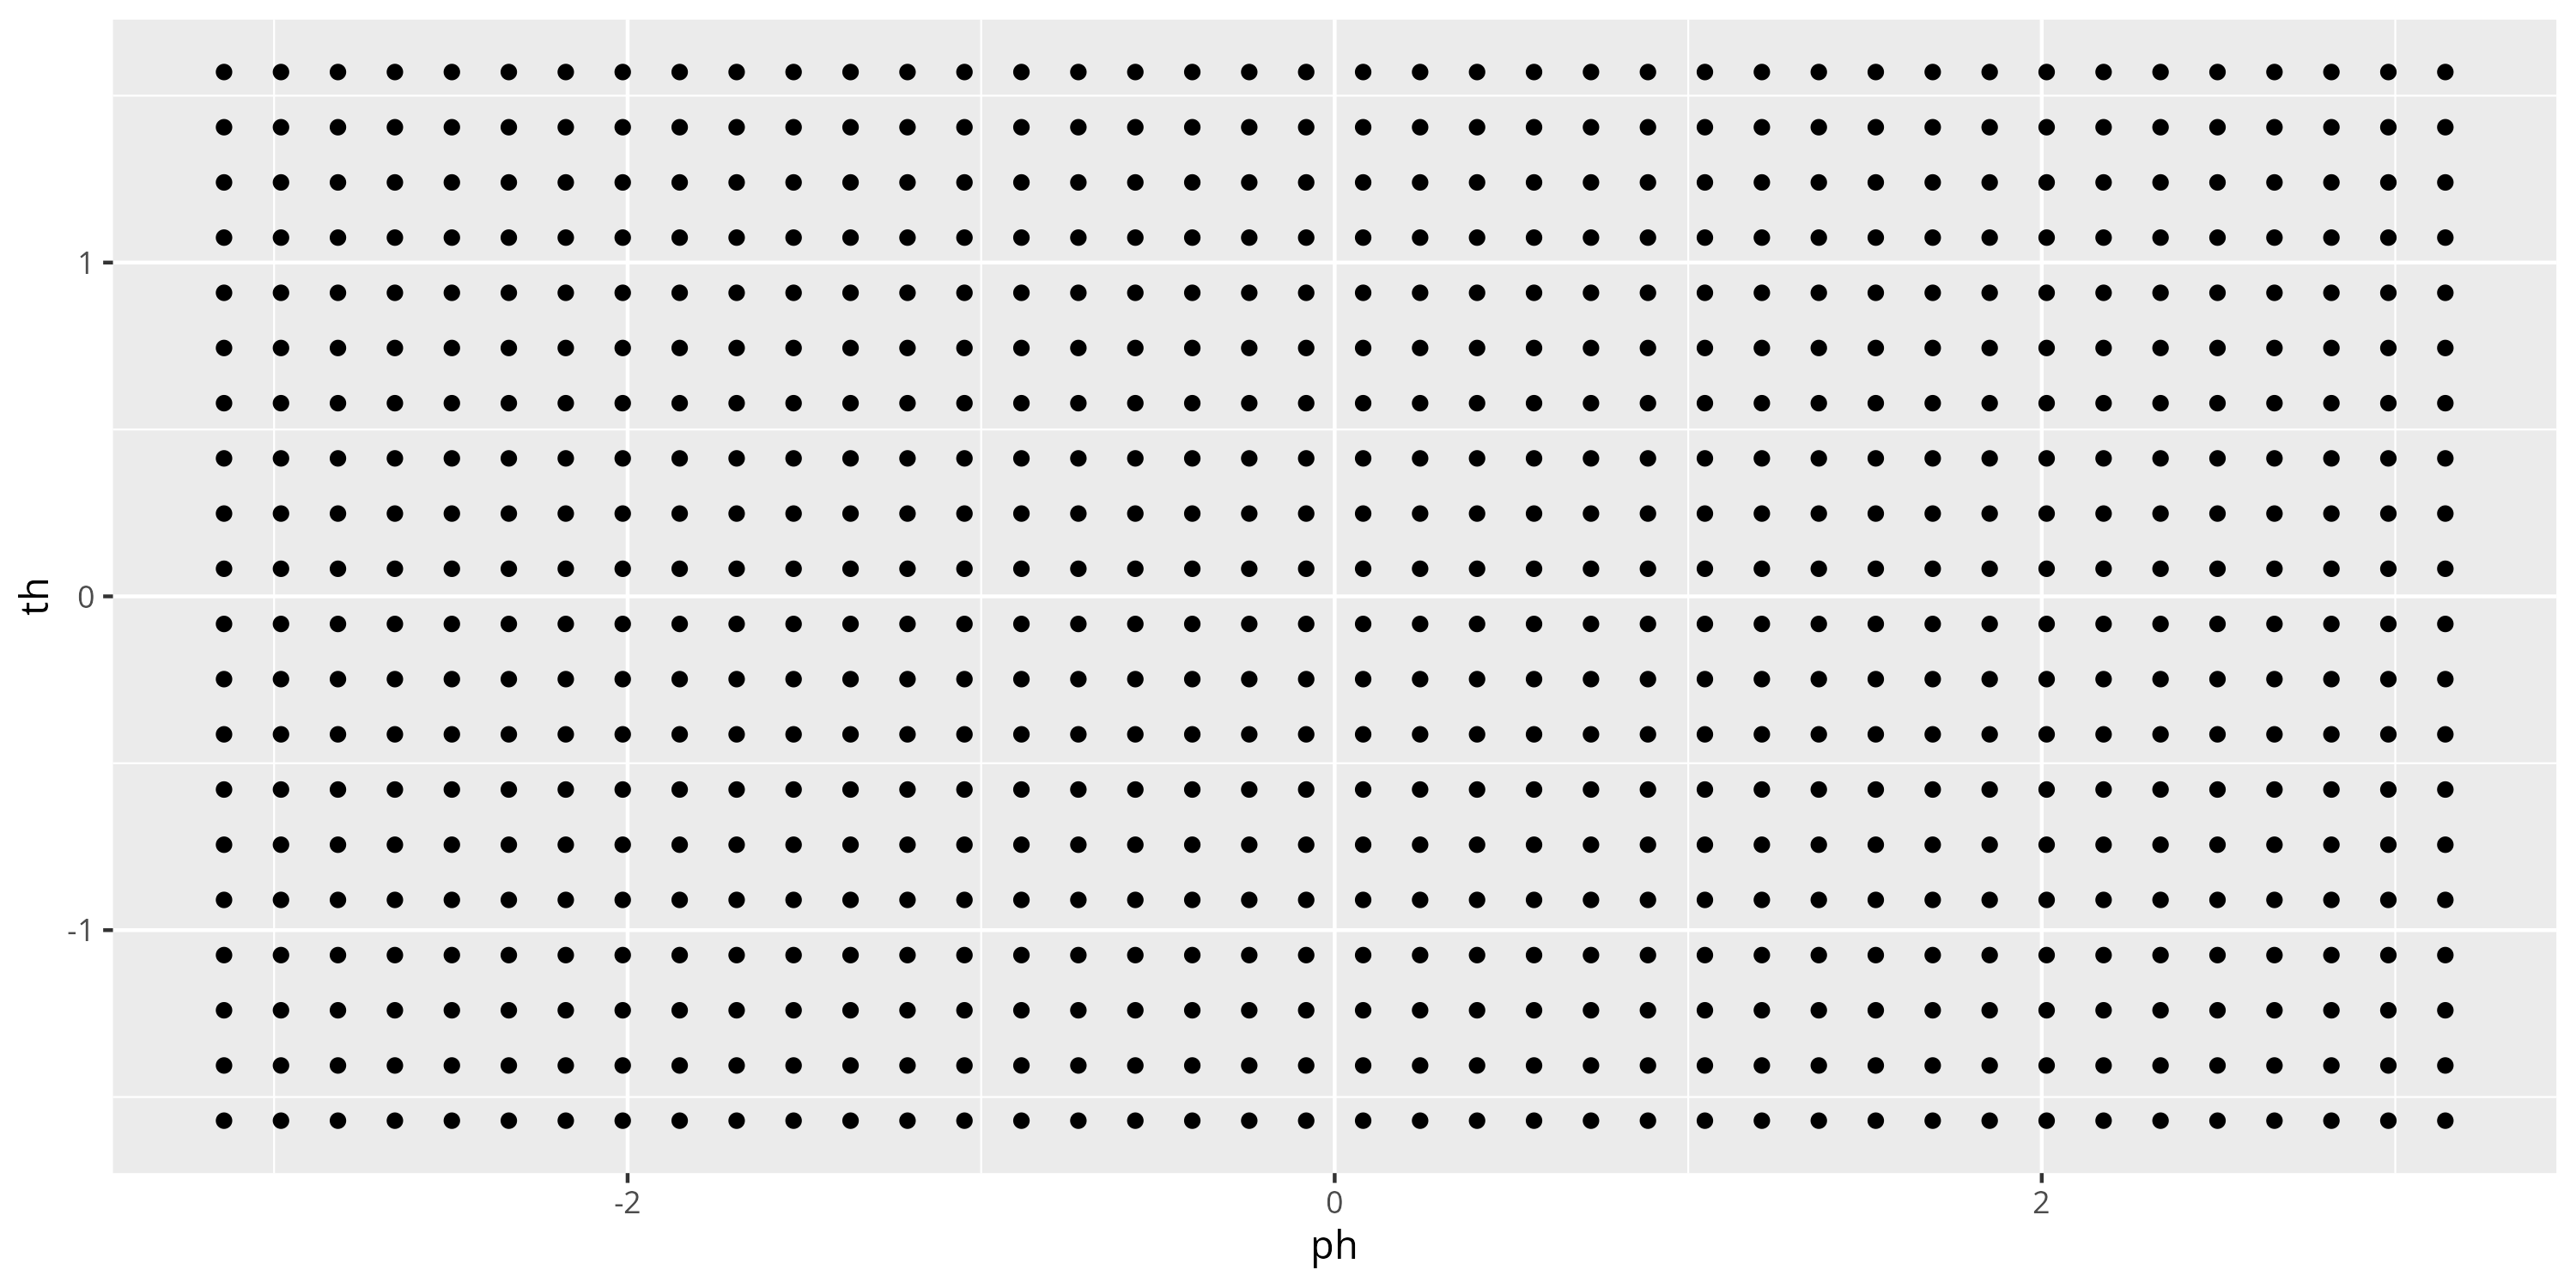
\includegraphics[width=.95\linewidth]{media/discretized_grid.png}
    %   \captionof{figure}{A figure}
      \label{fig:test1}
    \end{minipage}%
    \begin{minipage}{.5\textwidth}
      \centering
      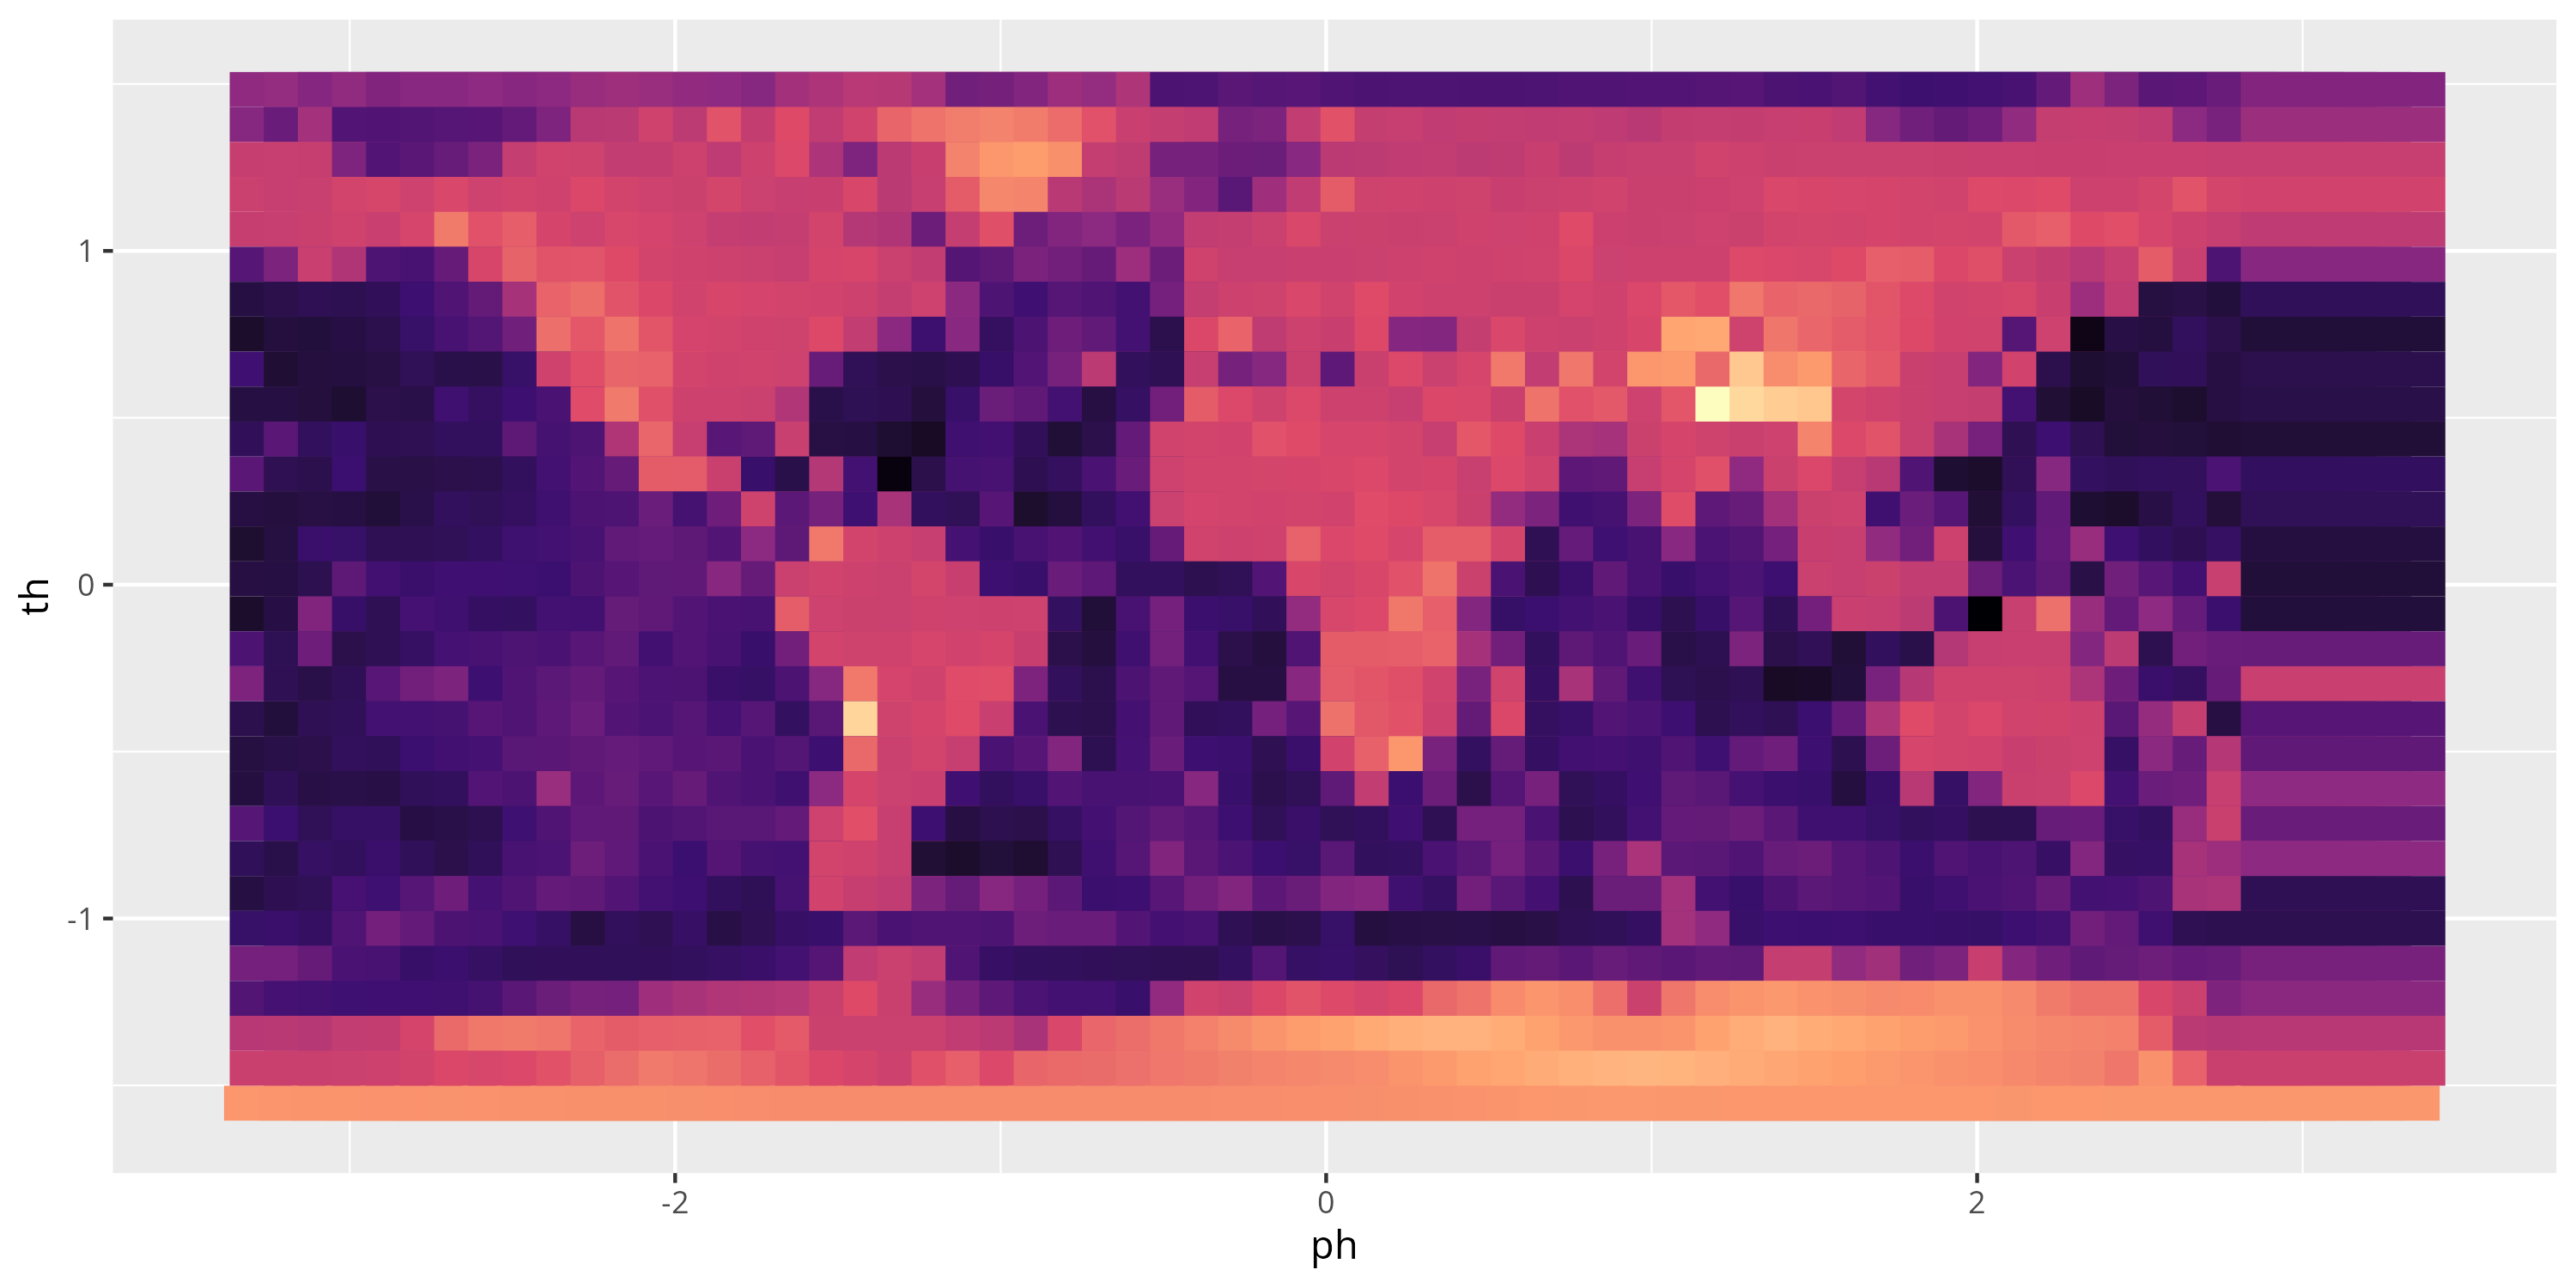
\includegraphics[width=.95\linewidth]{media/discretized_reduced.png}
    %   \captionof{figure}{Another figure}
      \label{fig:test2}
    \end{minipage}
    \caption{Discretization points (left) of a reduced data set with $n_\theta = 20$, $n_\phi = 40$. On the vertical axis we have $\theta \in [-\pi/2, \pi/2]$, or the latitude; On 
    the horizontal axis we have $\phi \in [-\pi, \pi]$, the longitude.}
\end{figure}

Due to the linear spacing, we only need to know the number of points $n_\theta$ and $n_\phi$ to recreate the spherical coordinate pairs provided 
by the data sets, allowing us to decrease the running memory footprint of our program. In order study informative analytics about our model, we first enumerate
the characteristics of each data set.

% \begin{figure}[h!]
    % \centering a
    \begin{center}
    \begin{tabular}{ c |  c  c  c }
        & $n_\theta$ & $n_\phi$ & $N$ \\ 
    \hline
    small & 180 & 360 & 64800\\
    med & 540 & 1080 & 583200\\
    hi \\
    ultra
    \end{tabular}
    \end{center}
% \end{figure}
$$\theta \in [0, \pi],\ \ \phi \in [0, \pi2]$$

We'll use these values later when we study the time it takes to compute our model.

\subsection{Visualization}

\textbf{TODO:} [ ] add 3-d maps

\section{Mathematical Model}




\subsection{Coefficients}

The coefficients $C_l^m$ and $S_l^m$ are defined as the orthogonal projection of $f(\theta, \phi)$ onto the basis functions $Y_l^m$, the spherical harmonics of degree $l$ and order $m$. This definition is perfectly analagous to the 
computation of fourier coefficients for $2\pi$ periodic functions. Written in terms of the associated legendre polynomials, these integrals are defined as

\begin{align*}
    \label{eq:coeff}
    C_l^m &= \int_0^{2\pi}\int_0^\pi f(\theta, \phi) P_l^m (\cos \theta)\cos (m \phi) \sin \theta d\theta d\phi\\
    S_l^m &= \int_0^{2\pi}\int_0^\pi f(\theta, \phi) P_l^m (\cos \theta)\sin (m \phi) \sin \theta d\theta d\phi 
\end{align*}

Taking advantage of the structure of the data sets, we approximate these coefficients via numerical quadrature.

\subsubsection{Computation via Numerical Integration}


    
We approximate the Laplace Series coefficients via a 2 dimensional analogue of the rectangle rule.  
\begin{align*}
    C_l^m &\approx \sum_{i = 1}^{n_\phi}\sum_{j = 1}^{n_\theta} f(\theta_j, \phi_i) P_l^m (\cos \theta_j)\cos (m \phi_i) \sin \theta_j \Delta\theta \Delta\phi\\
          &\approx \Delta\theta \Delta\phi\sum_{i = 1}^{n_\phi}\cos (m \phi_i)\sum_{j = 1}^{n_\theta} f(\theta_j, \phi_i) P_l^m (\cos \theta_j) \sin \theta_j\\
\end{align*}

\begin{align*}
    S_l^m &\approx \sum_{i = 1}^{n_\phi}\sum_{j = 1}^{n_\theta} f(\theta_j, \phi_i) P_l^m (\cos \theta_j)\sin (m \phi_i) \sin \theta_j \Delta\theta \Delta\phi\\
          &\approx \Delta\theta \Delta\phi\sum_{i = 1}^{n_\phi}\sin (m \phi_i)\sum_{j = 1}^{n_\theta} f(\theta_j, \phi_i) P_l^m (\cos \theta_j) \sin \theta_j\\
\end{align*}

This method computes \textit{individual} Laplace series coefficients in $O(N)$ time! Thus, computing the coefficients for a Discrete Laplace Series (DLS) of order $l_max$ runs in
$O(Nl^2_{max})$. More interestingly, each $C_l^m$ or $S_l^m$ can be computed \textbf{independently} of any other coefficient. Whereas solving the linear least squares problem requires computing
every $C_l^m$ and $C_l^m$ in a single operation, this method allows us the ability to compute any arbitrary $C_l^m$ directly. Why do we care? If I alraedy have the first 500 $C_l^m$ coefficients computed
and stored in a text file, I can \textit{directly} compute the 501st in $O(N)$ time. Furthermore, this method gives rise to obvious and easy-to-implement parallelization schemes.


\subsection{Comparison with Linear Squares}

Let's start by exploring the small data set and gathering data for how long it takes to compute a model.

\begin{figure}[h!]
    \centering
    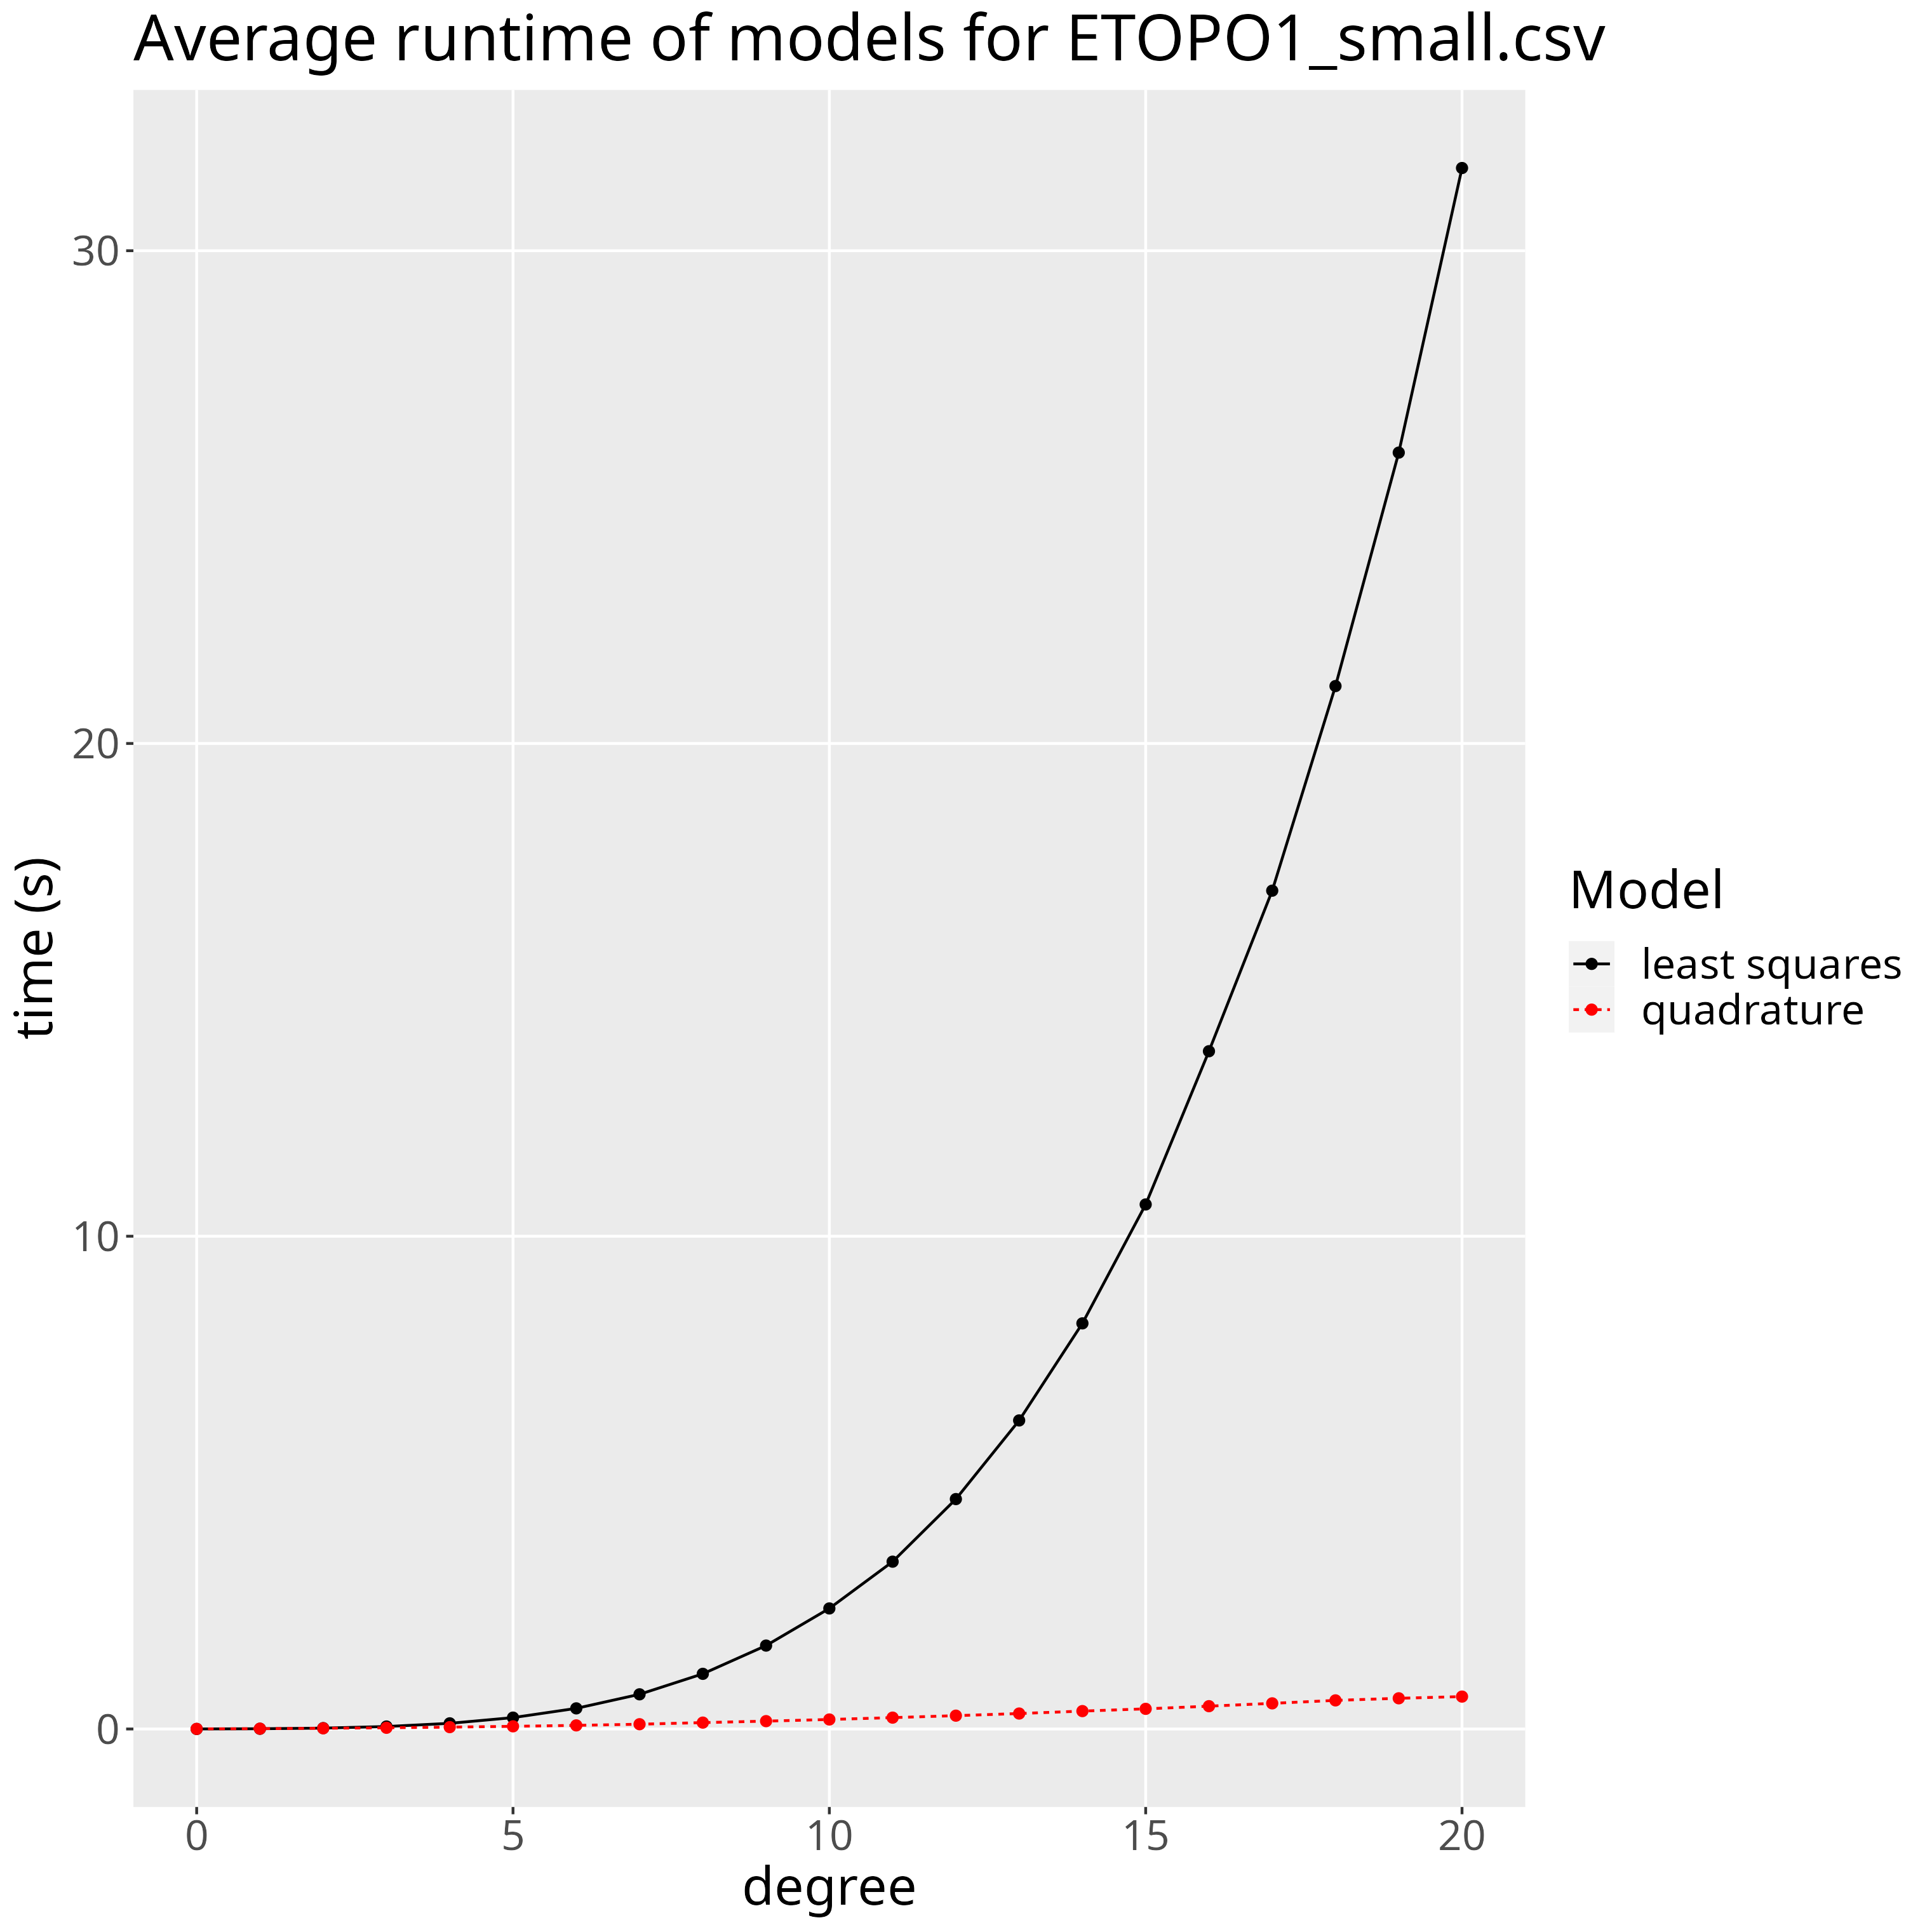
\includegraphics[width=0.6\textwidth]{media/average_runtime.png}
\end{figure}


Tested on the \verb|ETOPO1_small.csv| data set with $l_{max} = 20$, the model computed via numerical integration had an average error of about 2 times that of the least squares approach, but ran over 100 times faster.

\textbf{TODO}
\begin{itemize}
    \item Provide more detailed numeric comparison
    \item Provide timing analysis
\end{itemize}

\begin{figure}
    \centering
    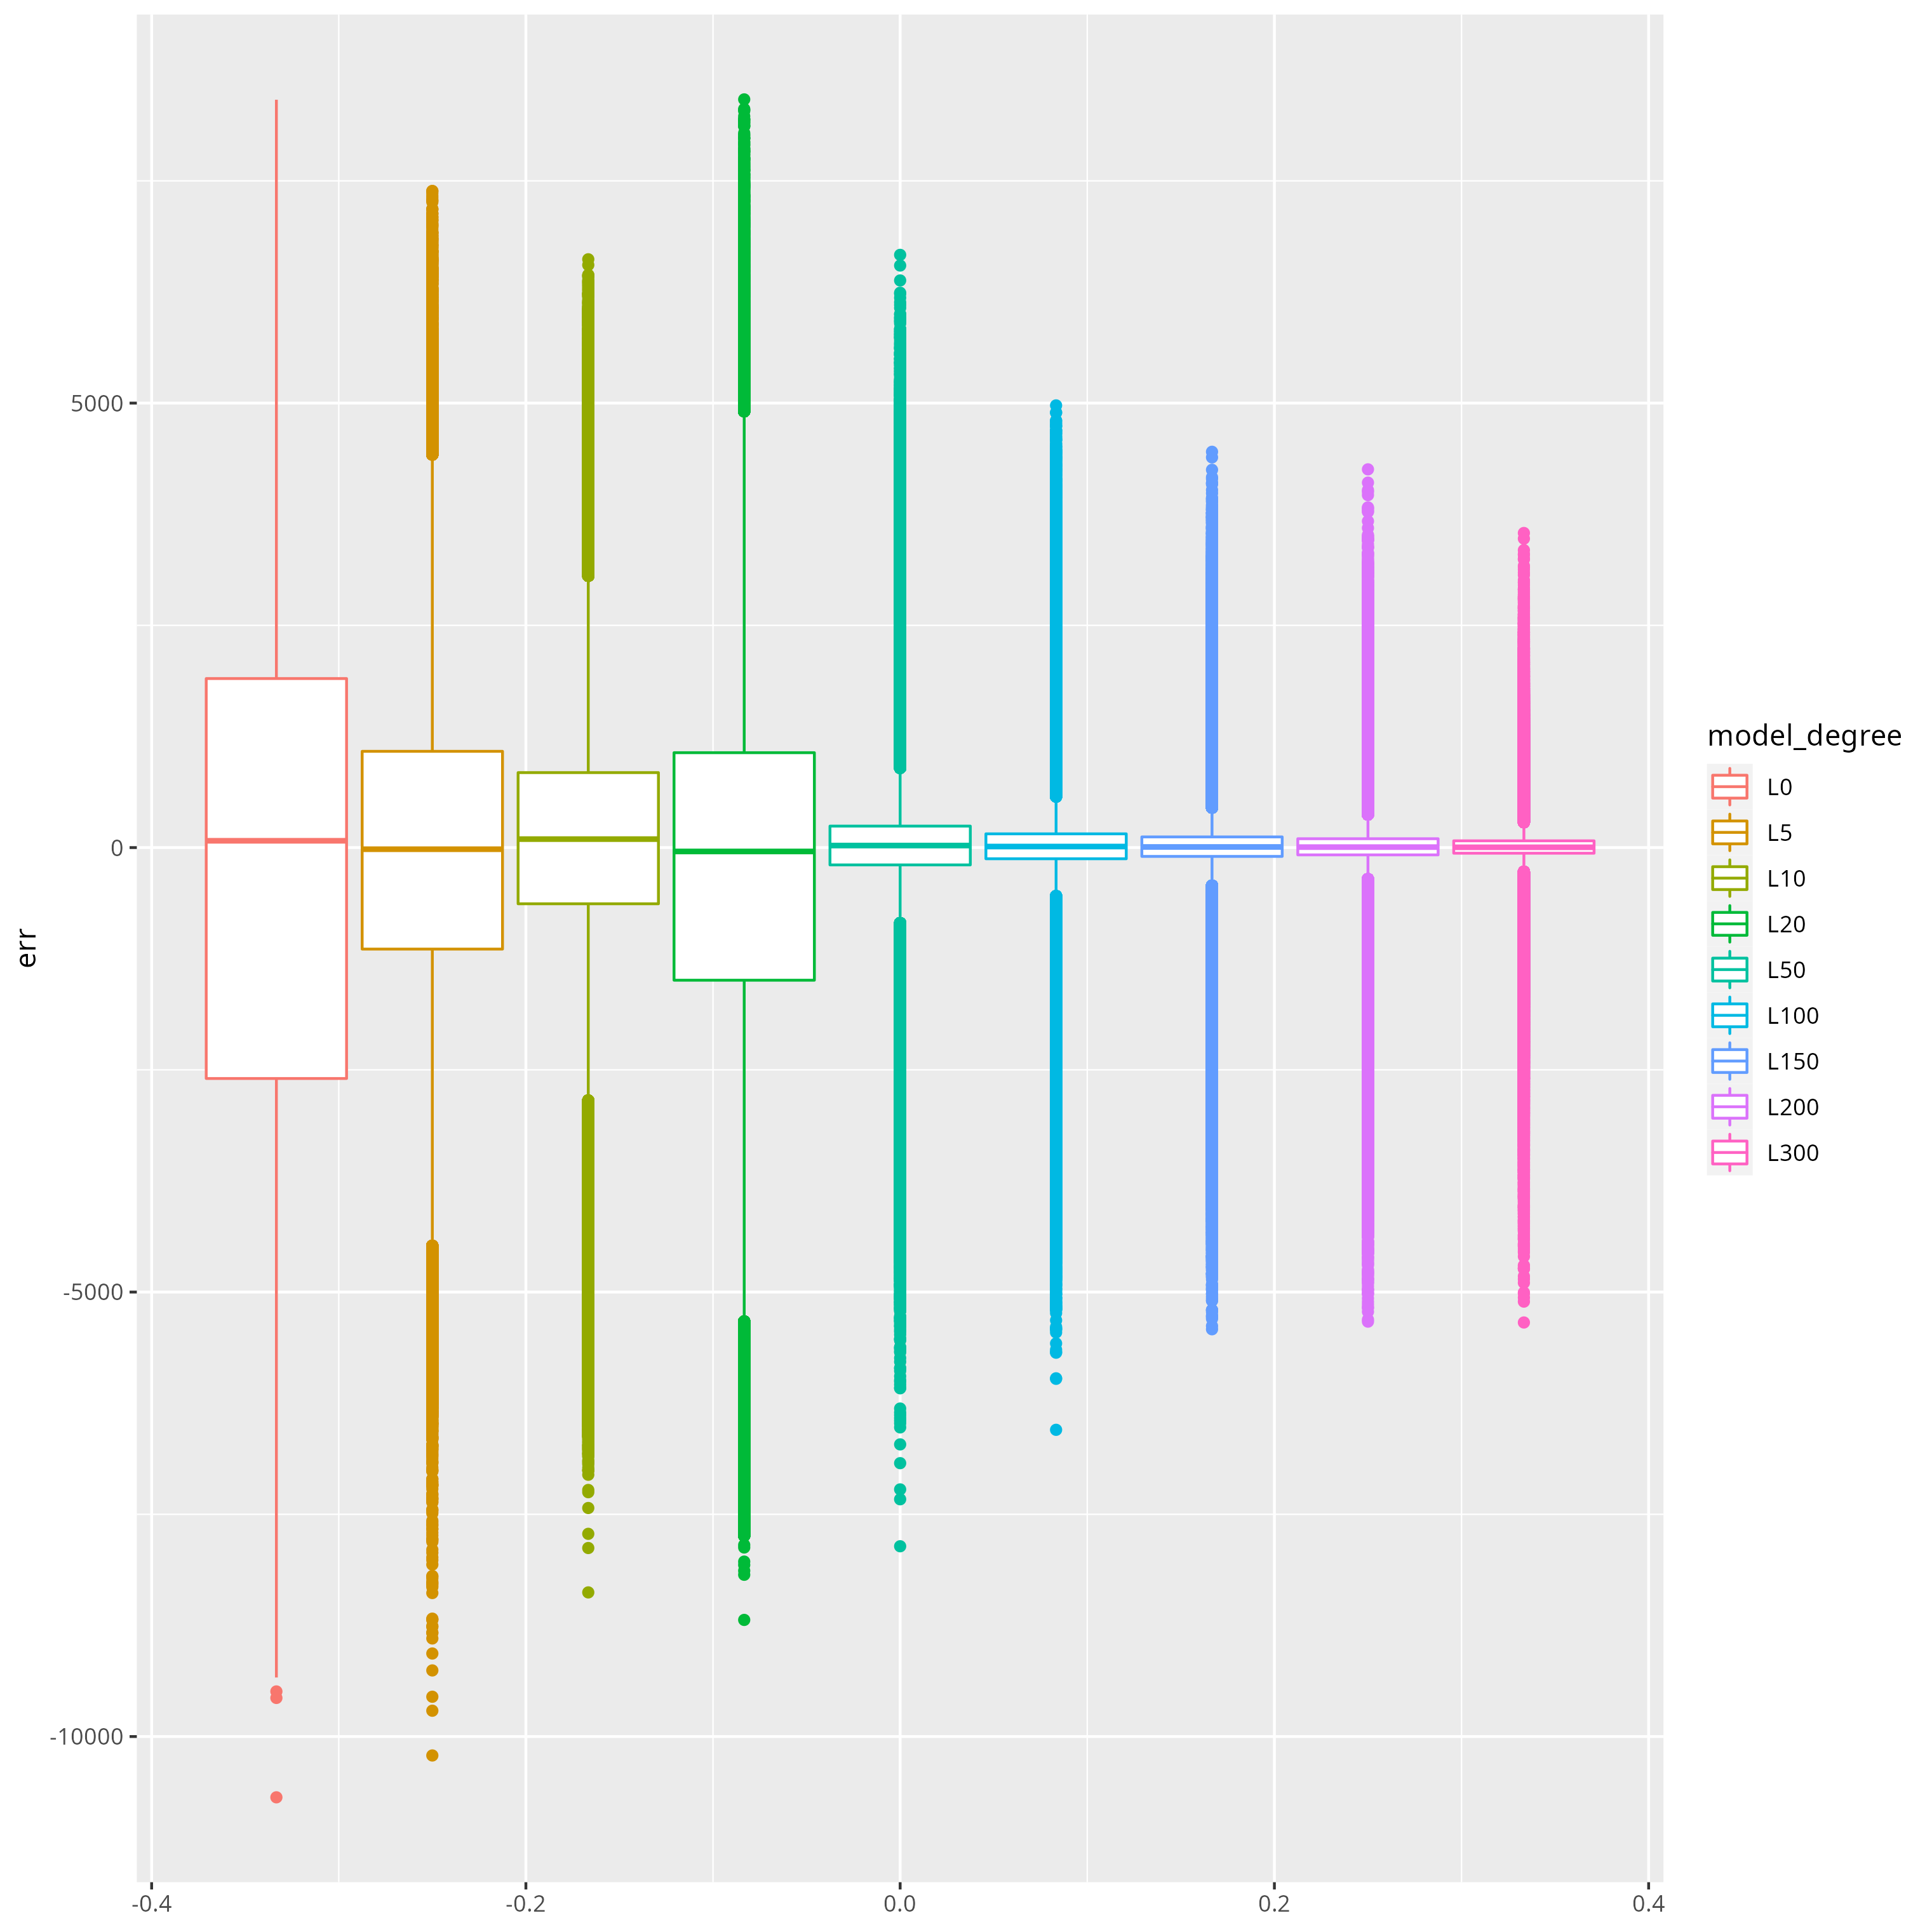
\includegraphics[width=0.5\linewidth]{media/boxplot_hi.png}
\end{figure}

\begin{figure}
    \centering
    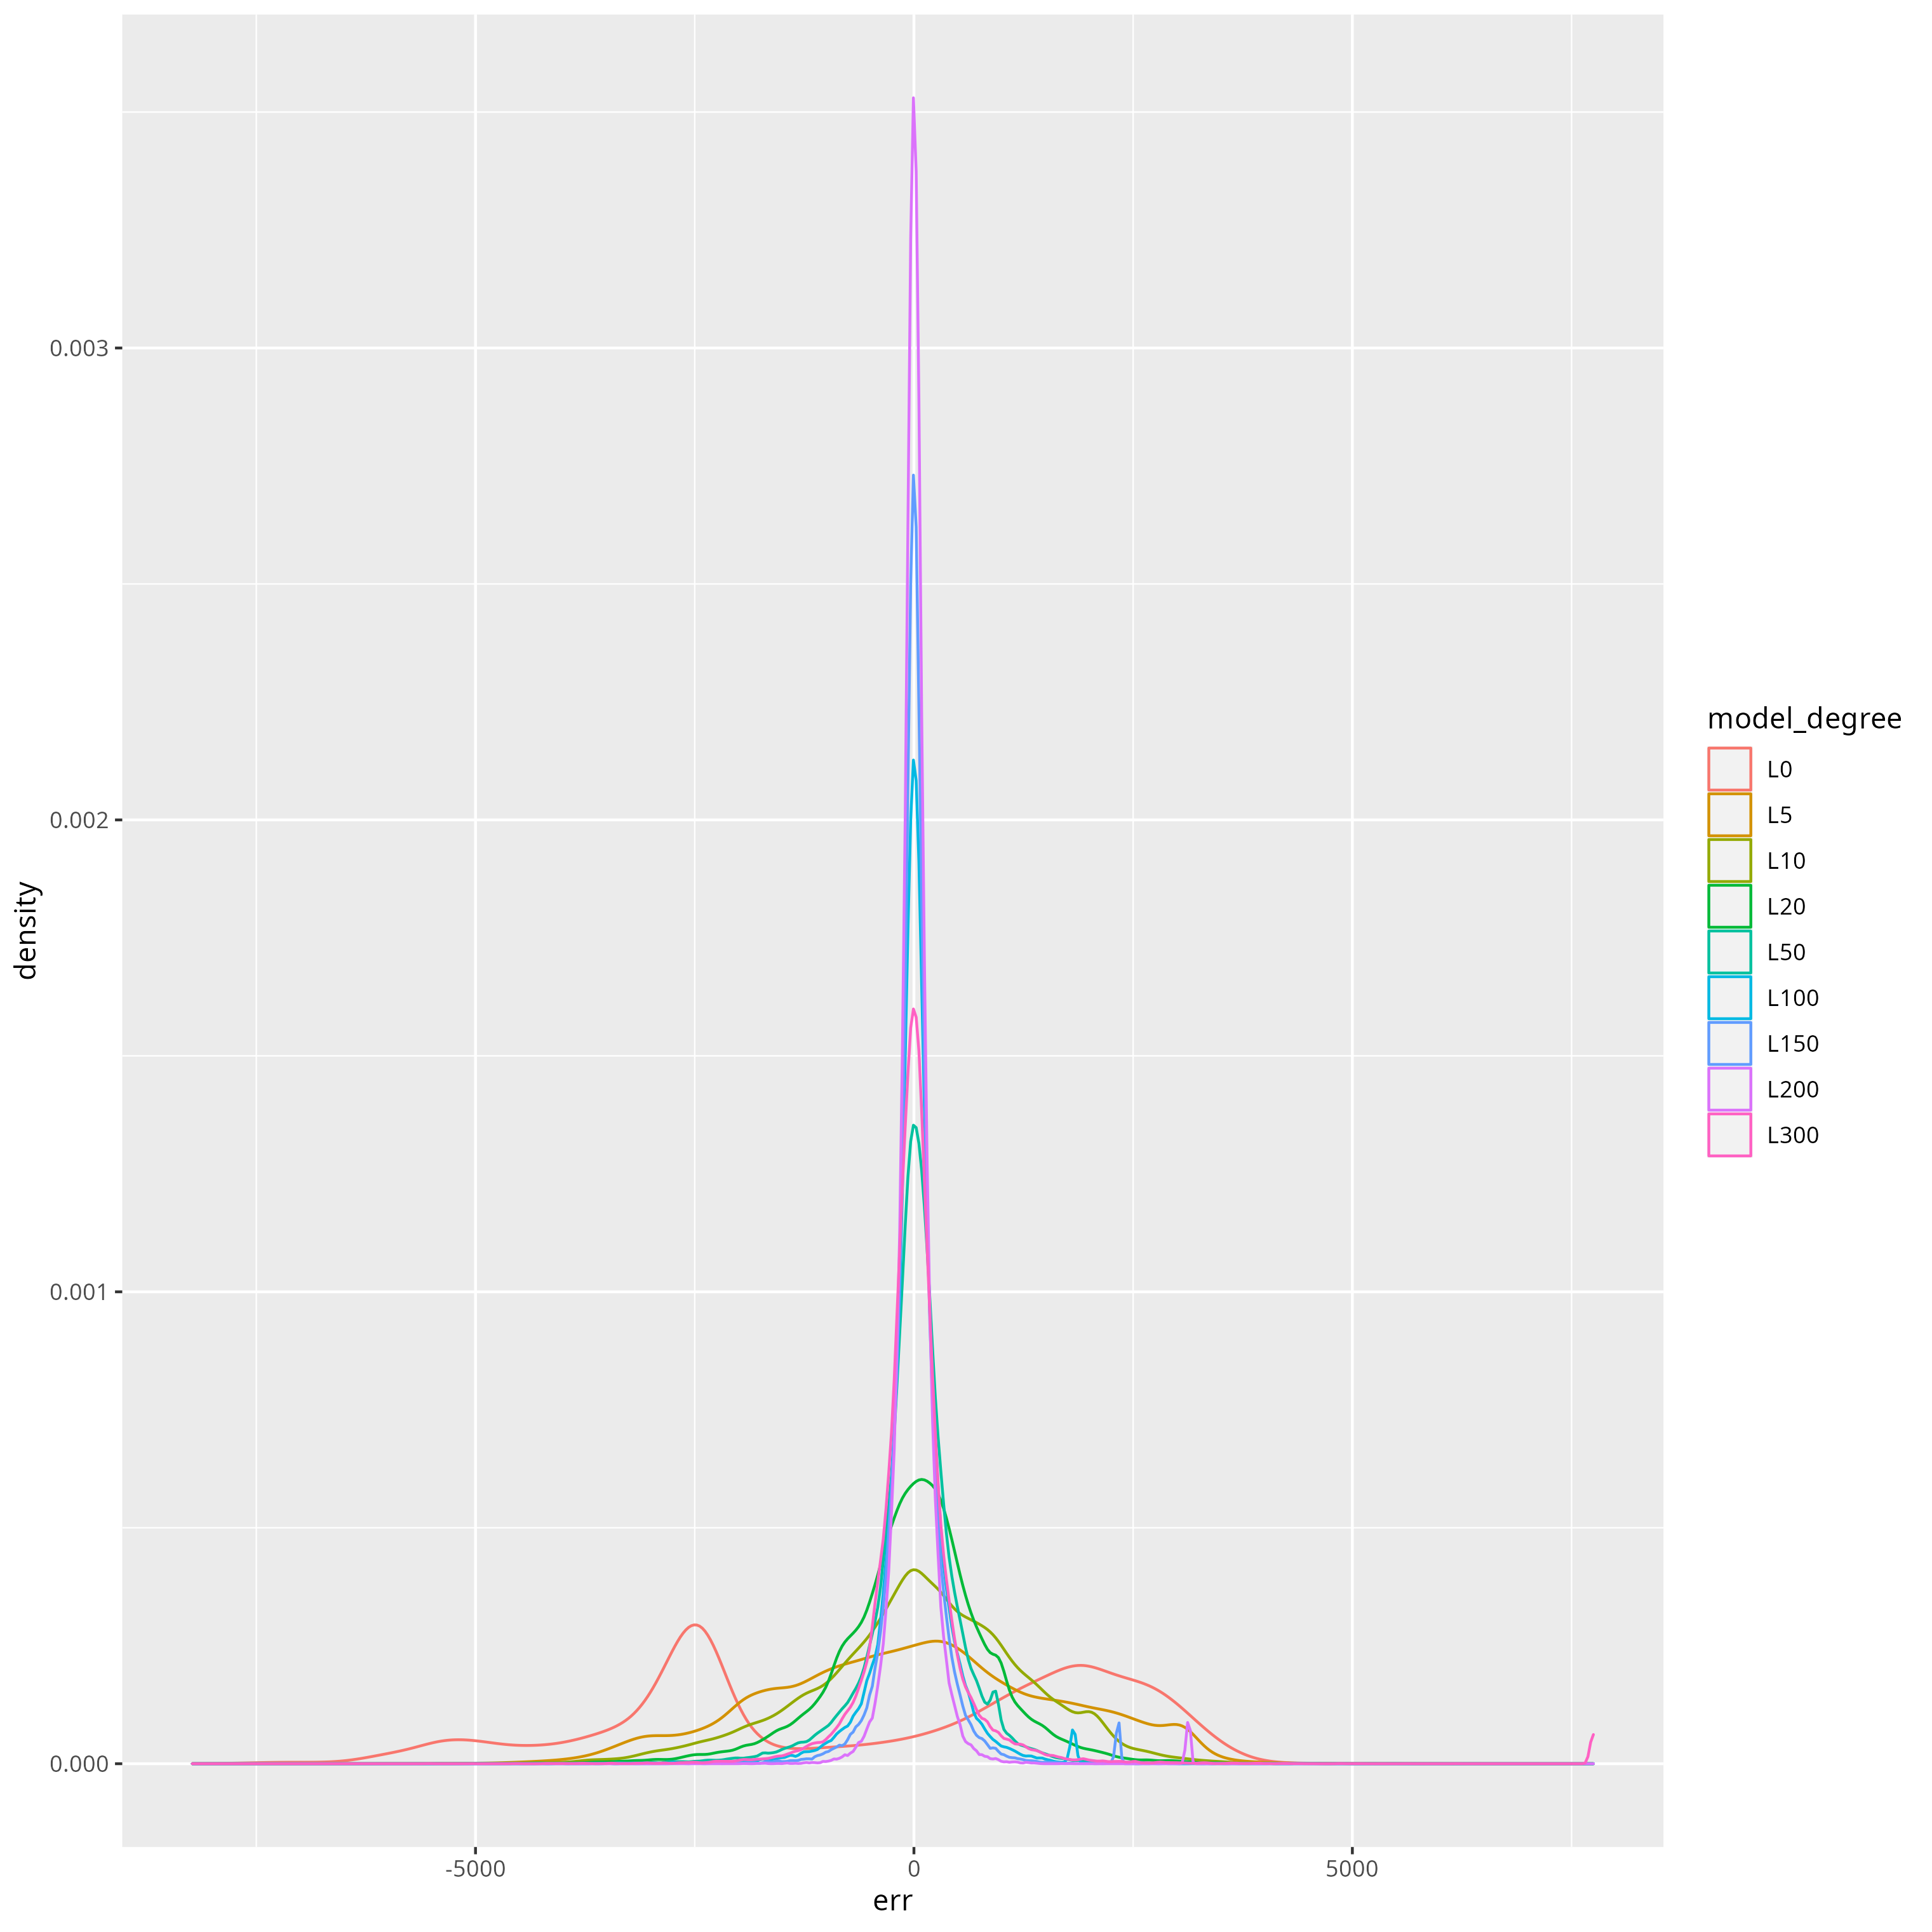
\includegraphics[width=0.5\linewidth]{media/density_small.png}
\end{figure}

\begin{figure}
    \centering
    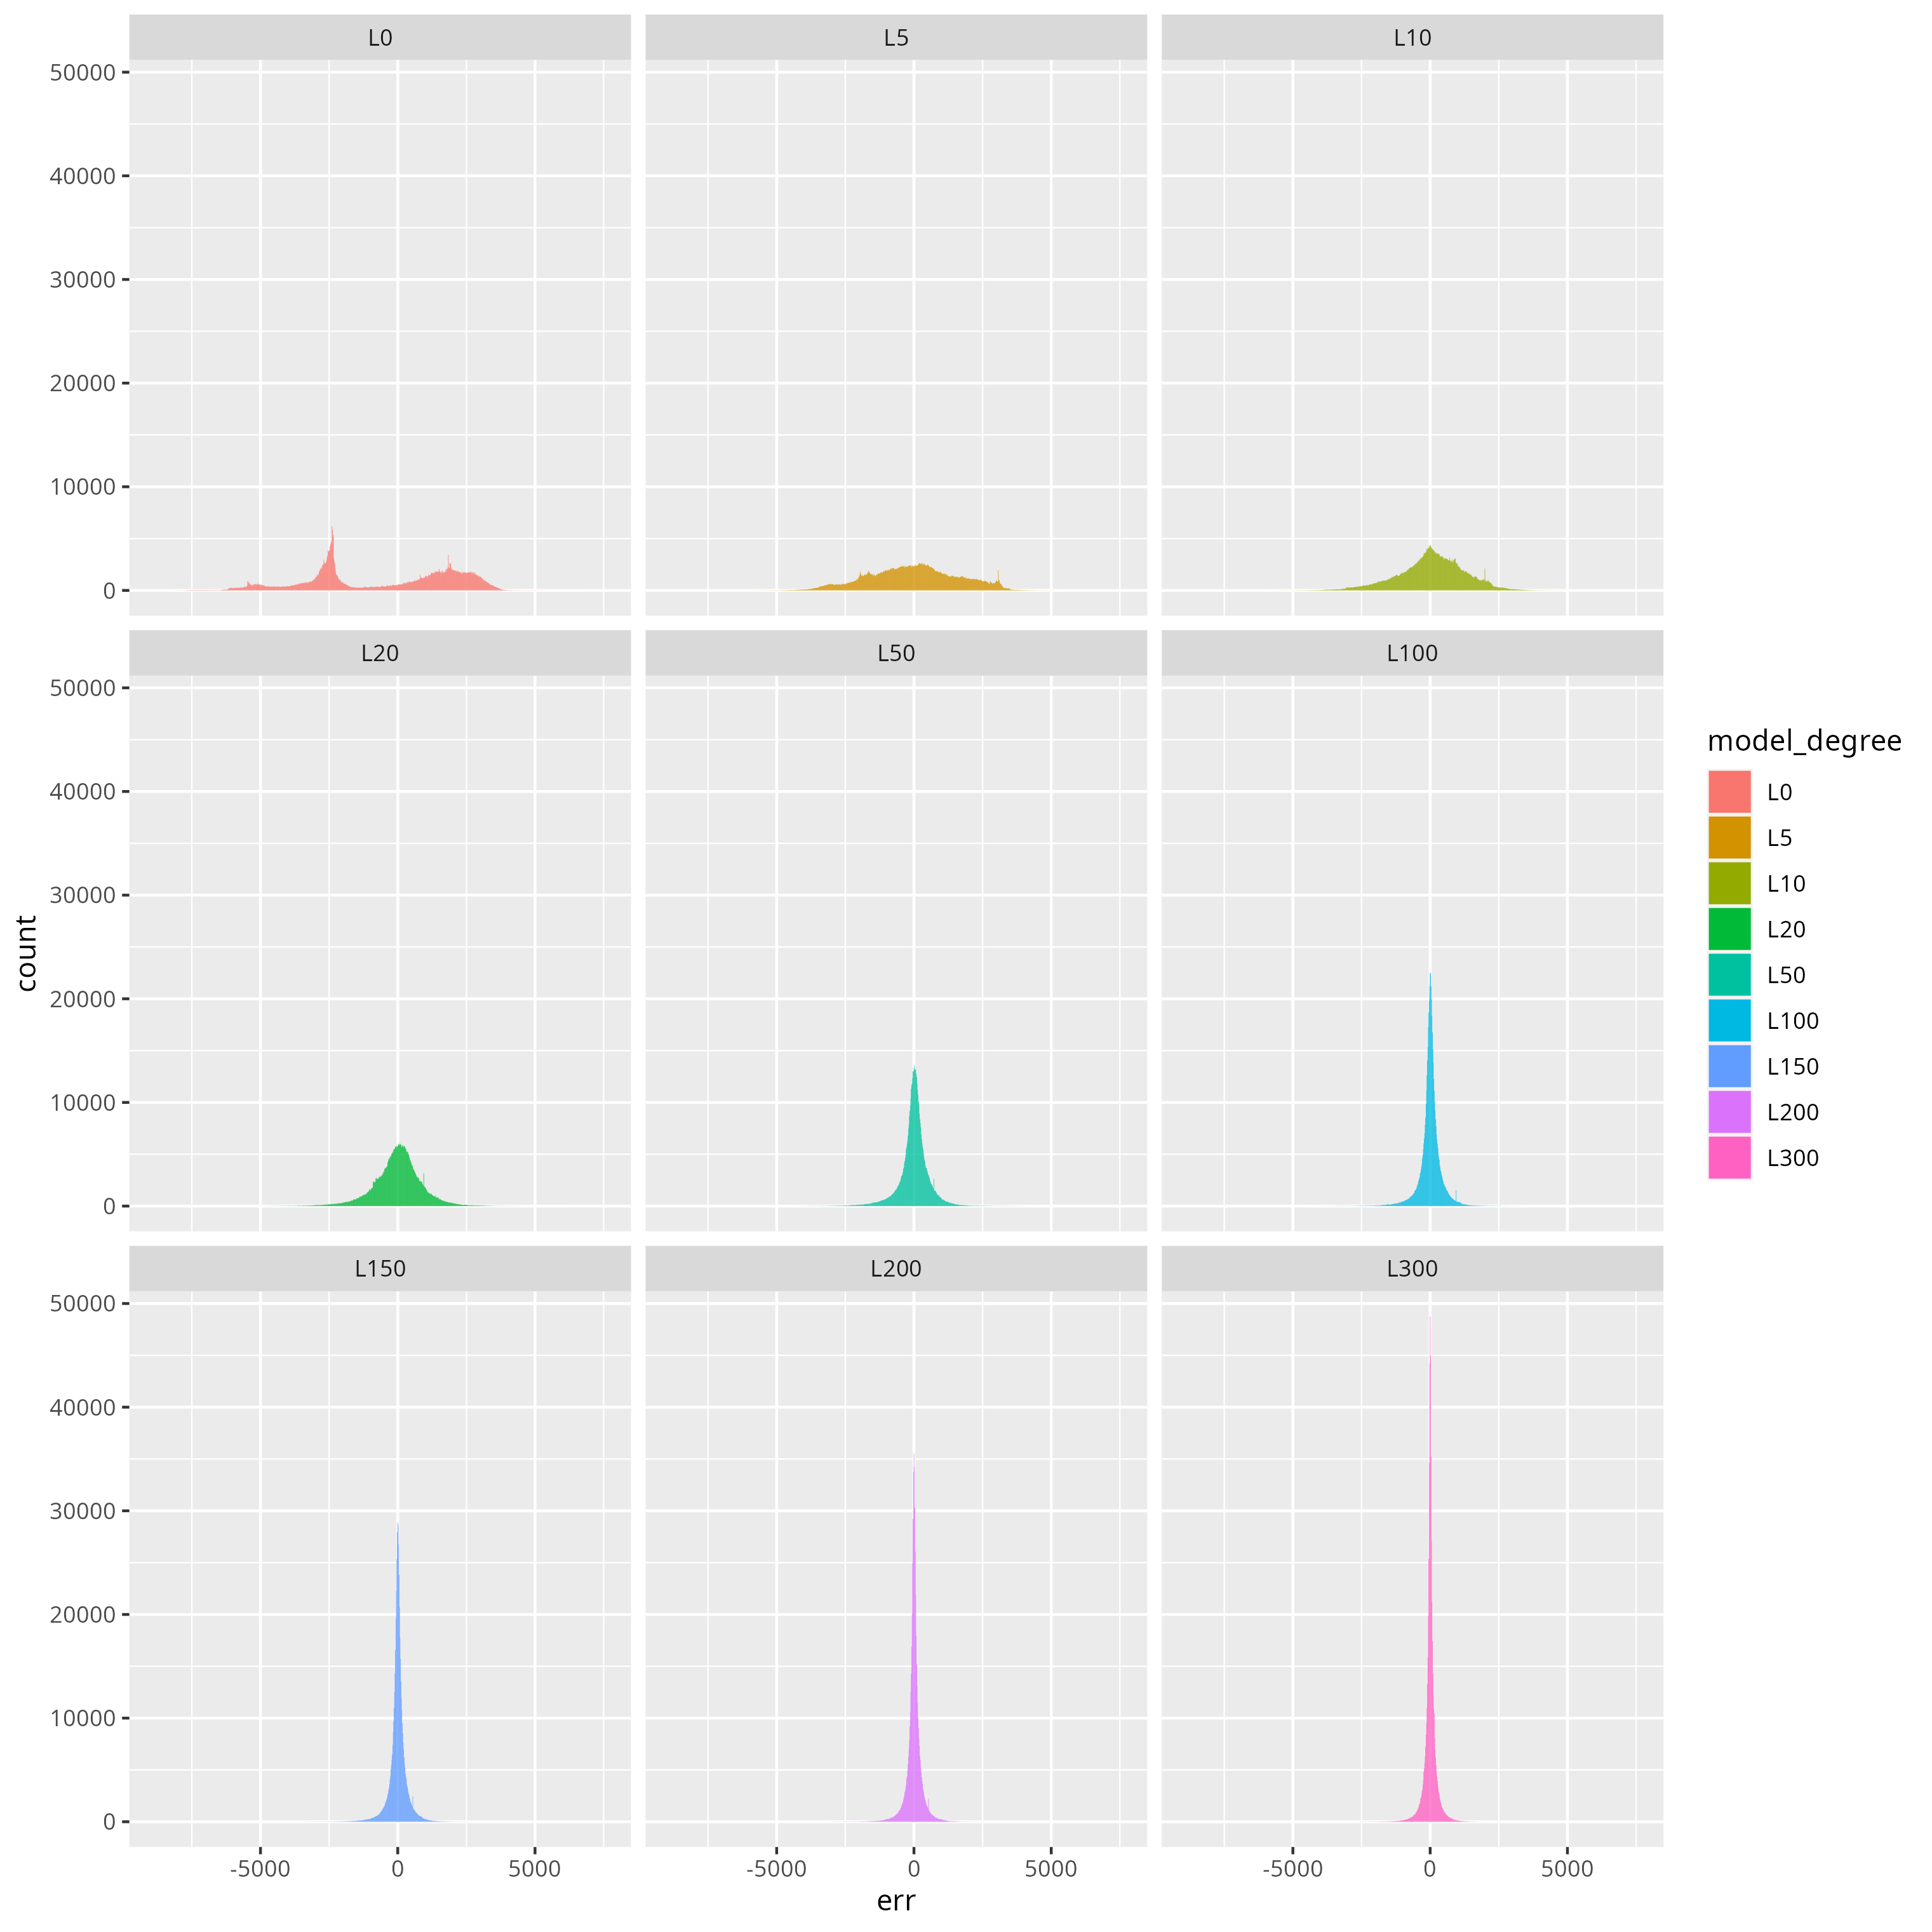
\includegraphics[width=0.5\linewidth]{media/faceted_histogram_med.png}

\end{figure}

section

\section{Improvements to the model}

The least squares method provides a more accurate model, but runs in $O(Nl^4_{max})$ time. In this section we propose improvements to our model computed via quadrature.

\subsection{Gradient Descent}

We can apply methods of optimization to minizmize the mean squared error (MSE) of our model. To begin we explicitze the MSE then compute its gradient



\textbf{TODO} I have already derived the gradient of the MSE with respect to all $C_l^m$ and $S_l^m$ on paper
\begin{itemize}
    \item Write up derivation in latex
\end{itemize}

Computing the gradient vector runs in \textcolor{red}{$O(Nl_{max}^2)$} time


\subsubsection{Stochastic Gradient Descent}

Computing the gradient with respect to a single $C_l^m$ requires summing up certain values for all $N$ points of the data set. For larger data sets (e.g. $N_{high} = 1800 * 3600 = 6480000$), this
computation can become intractable. We can speed up our gradient computation by computing as estimate of the gradient, $\hat\nabla$MSE, by randomly sampling $n$ points from our entire
data set. This reduces the computation of a gradient vector from $O(Nl_{max}^2)$ to \textcolor{red}{$O(nl_{max}^2)$}. This is an \textbf{insane} improvement to the run time of our algorithm.
Instead of summing all 6480000 points of the large data set, we could fix $n$ at say $n = 1000$ instead, sacrificing accuracy for a speedeup of 6,480.

\subsection{MCMC Algorithms}

In initial tests my gradient descent learning is \textit{sometimes} reducing the MSE but other times it's increasing it... If I don't figure out exactly what's going wrong 
then I plan on implementing MCMC algorithms like Gibb's sampling to explore the sample space and only accept proposal vectors that decrease the MSE.

\section{Parallelization} 

\textbf{TODO} (trivial)

\section{Conclusion}

Instead of calculating the model with a direct method that runs in $O(Nl_{max}^4)$ time, We propose a hybrid model that first directly computes the coefficients in $O(Nl_{max}^2)$ time then 
iteratively improves the MSE via stochastic methods running in $O(n_{training}n_{sample}l_{max}^2)$ time.

Results are to follow :)





\appendix
\section{Spherical Coordinates Transformation}

The data sets \verb|ETOPO1_*.csv| provided by NASA represent spherical coordinates in an unconventional format: $$(\phi, \lambda) \in [-\frac{\pi}{2}, \frac{\pi}{2}] \times [-\pi, \pi] $$ where $\phi$ refers to the latitude
and $\lambda$ refers to the longitude. In this section we outline the transformation from NASA's coordinate system to the ISO standard representation and prove equivalence between (1) and the Project presentation's $f(\phi, \lambda)$.

To avoid confusion, we denote the spherical coordinate pair in ISO coordinates as $(\theta_{iso}, \phi_{iso})$ and NASA's coordinate scheme as $(\phi_{nasa}, \lambda_{nasa})$.
We remark that the polar angle $\theta_{iso}$ is simply equal to $\frac{\pi}{2} - \phi_{nasa}$. We corroborate this fact by remarking that a latitude of $\phi_{nasa} = 0$ corresponds to a polar
angle of $\phi_{iso} = \frac{\pi}{2}$. Conveniently, the longitude $\lambda_{nasa}$ is equivalent to the azimuthal angle $\phi_{iso}$.

\begin{proposition} Let the spherial coordinate pairs $(\theta_{iso}, \phi_{iso})$, $(\phi_{nasa}, \lambda_{nasa})$ be defined as above. 
    \begin{equation*}
        f(\theta_{iso}, \phi_{iso}) \equiv f(\phi_{nasa}, \lambda_{nasa})
    \end{equation*}

    
\end{proposition}



\begin{proof}
    $f(\phi_{nasa}, \lambda_{nasa})$ is defined in the Project proposal as 
    \begin{align} \label{eq:project_def} 
        f(\phi_{nasa}, \lambda_{nasa}) &= \sum_{l = 0}^{+\infty}\sum_{m = 0}^l \bar P_l^m(\sin\phi_{nasa})[C_l^m\cos m\lambda_{nasa} + S_l^m \sin m \lambda_{nasa}] \\ 
                                       &= \sum_{l = 0}^{+\infty}\sum_{m = 0}^l \bar P_l^m(\sin(\pi/2 - \theta_{iso}))[C_l^m\cos m\phi_{iso} + S_l^m \sin m \phi_{iso}] \\
                                       &= \sum_{l = 0}^{+\infty}\sum_{m = 0}^l \bar P_l^m(\cos\theta_{iso}))[C_l^m\cos m\phi_{iso} + S_l^m \sin m \phi_{iso}] \\
                                       &\equiv f(\theta_{iso}, \phi_{iso})
    \end{align}

\end{proof}

\nocite{*}

\bibliography{ppar}
\bibliographystyle{ieeetr}

\end{document}

